\documentclass[tikz,border=6pt]{standalone}
\usetikzlibrary{arrows.meta,angles,quotes,calc,intersections,positioning}


\definecolor{ksupurple}{HTML}{512888}
\definecolor{orange}{HTML}{CA7C1B}
\begin{document}
% requires: \usetikzlibrary{arrows.meta}
%\begin{minipage}{0.48\textwidth}

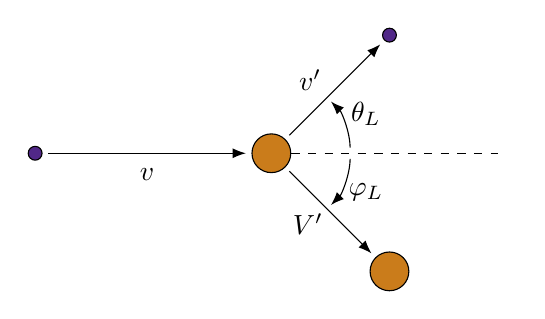
\begin{tikzpicture}[x=1.5cm,y=1.5cm,>=Latex]

  \node[circle,draw,fill=ksupurple,minimum size=5pt,inner sep=0pt] (a) at (-2,0) {};
  \node[circle,draw,fill=orange,minimum size=14pt,inner sep=0pt]   (b) at (0,0) {};
  \draw[->,shorten <=2pt,shorten >=2pt]
    (a) -- (b) node[midway,below=2pt] {$v$};
  \node[circle,draw,fill=ksupurple,minimum size=5pt,inner sep=0pt] (c) at (1,1) {};
  \node[circle,draw,fill=orange,minimum size=14pt,inner sep=0pt]   (d) at (1,-1) {};
  \node[] (e) at (2,0) {}; % dummy place holder
  \draw[->,shorten <=2pt,shorten >=2pt]
    (b) -- (c) node[pos=0.25,above=5pt] {$v'$};
  \draw[->,shorten <=2pt,shorten >=2pt]
    (b) -- (d) node[pos=0.25,below=5pt] {$V'$};
  \draw[-,dashed] (b) -- (e); % reference line
  \pic[draw,angle radius=10mm, ->, 
       angle eccentricity=1.3,"$\theta_{L}$",
       shorten <=2pt,shorten >=2pt] {angle = e--b--c};
  \pic[draw,angle radius=10mm, <-,
       angle eccentricity=1.3,"$\varphi_{L}$", 
       shorten <=2pt,shorten >=2pt] {angle = d--b--e};
\end{tikzpicture}

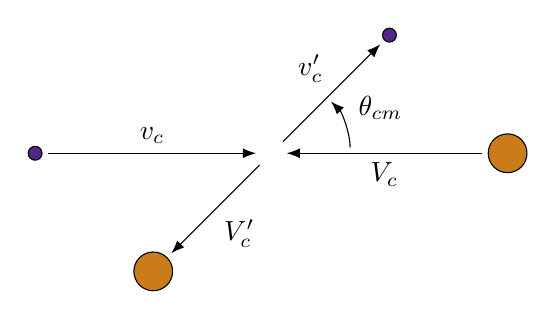
\begin{tikzpicture}[x=1.5cm,y=1.5cm,>=Latex]
  \node[circle,draw,fill=ksupurple,minimum size=5pt,inner sep=0pt] (a) at (-2,0) {};
  \node[circle,draw,fill=orange,minimum size=14pt,inner sep=0pt]   (b) at (2,0) {};
  \node[] (cm) at (0,0) {};
  \draw[->,shorten <=2pt,shorten >=2pt] (a) -- (cm) node[midway,above] {$v_c$};
  \draw[->,shorten <=2pt,shorten >=2pt] (b) -- (cm) node[midway,below] {$V_c$};
  \node[circle,draw,fill=ksupurple,minimum size=5pt,inner sep=0pt] (c) at (1,1) {};
  \draw[->,shorten <=1pt,shorten >=2pt] (cm) -- (c) node[midway,above left] {$v_c'$};
  \node[circle,draw,fill=orange,minimum size=14pt,inner sep=0pt] (d) at (-1,-1) {};
  \draw[->, shorten <=1pt,shorten >=2pt] (cm) -- (d) node[midway,below right] {$V_c'$};
  \pic[draw,angle radius=10mm, ->,
       angle eccentricity=1.5,"$\theta_{cm}$", 
       shorten <=2pt,shorten >=2pt] {angle = b--cm--c};
\end{tikzpicture}

\end{document}
